\begin{frame}[label = phogamma, t]{Phổ $\gamma$}

Phổ $\gamma$ thực nghiệm:

\setlength{\picW}{0.4\textwidth}
\setlength{\picH}{0.806\picW}
\setlength{\pit}{0.1\picW}

%\only<1-2>{
\begin{tikzpicture}
\only<3->{\clip(5\pit,0) rectangle (8\pit, 4\pit);}
\node at (0.5\picW, 0.5\picH){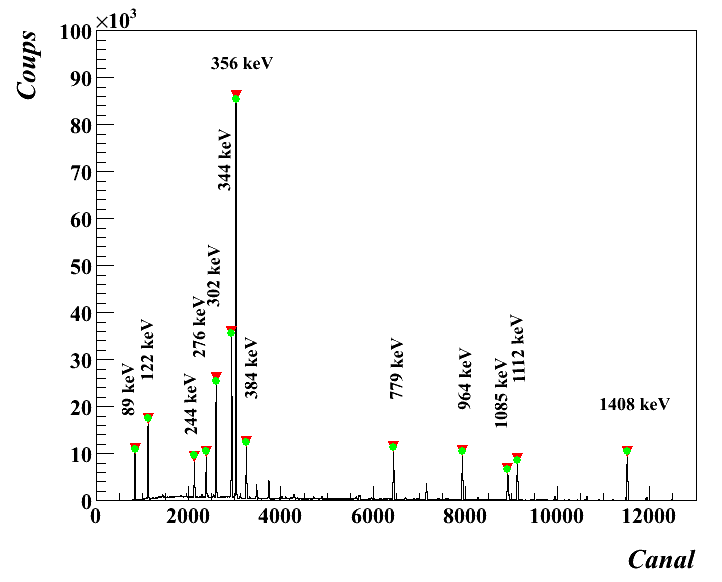
\includegraphics[width = \picW]{figure/phogamma.png}};
%\draw[gray!30](0,0) grid[step=\pit] (\picW, \picH);
\only<2-2>{\draw[line width = 1.5pt, color = red](6.5\pit,2\pit) circle (2\pit);}
\end{tikzpicture}
%}

%\only<3->{
%\scalebox{3}{
%\begin{tikzpicture}
%\clip(5\pit,0) rectangle (8\pit, 4\pit);
%\node at (0.5\picW, 0.5\picH){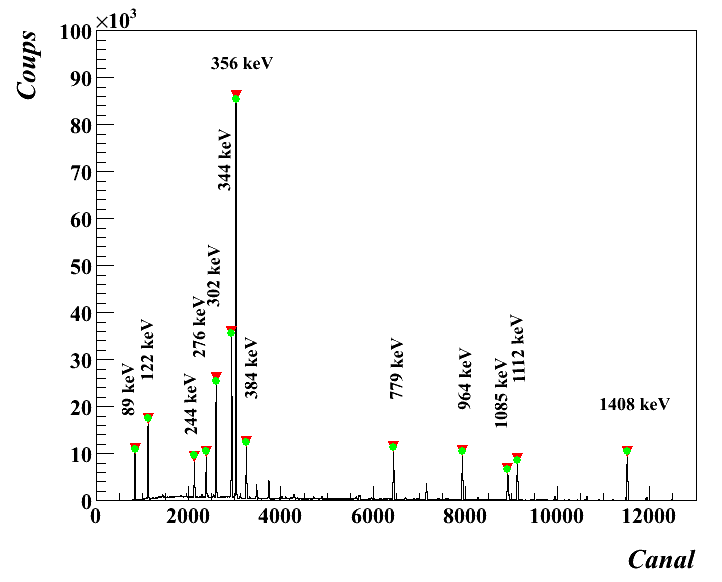
\includegraphics[width = \picW]{figure/phogamma.png}};
%%\draw[gray!30](0,0) grid[step=\pit] (\picW, \picH);
%%\draw[line width = 1.5pt, color = red](6\pit,3\pit) ellipse (1 and 2);
%\end{tikzpicture}
%}
%}

\end{frame}